\documentclass{article}
\usepackage{xcolor}
\usepackage{graphicx}
\usepackage{tikz}
\usepackage{circuitikz}
\usepackage{pgfplots}
\usepackage{darkmode}
\usepackage{amsmath}
\usepackage[a4paper, top=2cm, bottom=2cm]{geometry}

\enabledarkmode

\definecolor{c1}{HTML}{8bb6e7}
\definecolor{c2}{HTML}{87f3dd}
\definecolor{c3}{HTML}{fdef83}
\definecolor{c4}{HTML}{fdc373}
\definecolor{c5}{HTML}{fd8581}
\definecolor{c6}{HTML}{c573e7}
\definecolor{c7}{HTML}{afdb68}
\definecolor{c8}{HTML}{e59f8b}

\definecolor{page}{HTML}{262626}
\pagecolor{page}

\begin{document}
\title{Tarea Previa 4}
\author{Mario López Sáez}
\date{\today}
\maketitle

\begin{center}

\begin{tikzpicture}
    \fill[c1] (0, 0) rectangle ++(1, 0.05);
    \fill[c2] (1, 0) rectangle ++(1, 0.05); 
    \fill[c3] (2, 0) rectangle ++(1, 0.05);
    \fill[c4] (3, 0) rectangle ++(1, 0.05);
    \fill[c5] (4, 0) rectangle ++(1, 0.05);
    \fill[c6] (5, 0) rectangle ++(1, 0.05);
    \fill[c7] (6, 0) rectangle ++(1, 0.05);
    \fill[c8] (7, 0) rectangle ++(1, 0.05);
\end{tikzpicture}

\end{center}

\begin{center}
    {\large Amplificador con MOSFET}
\end{center}
\begin{figure}[h!]
    \centering
    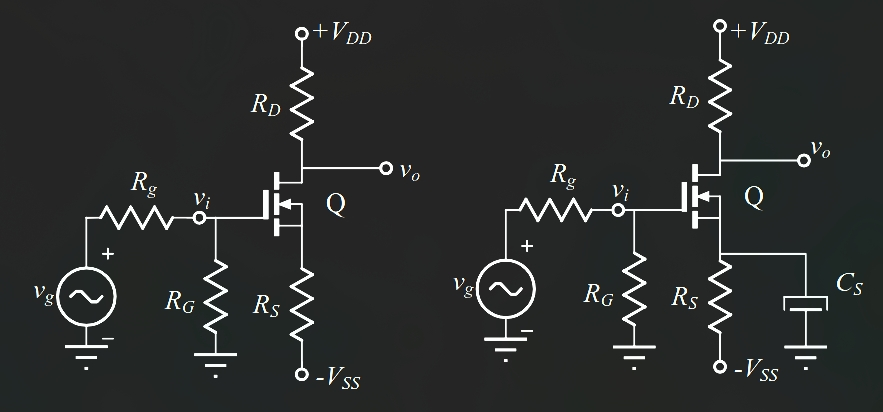
\includegraphics[width=1\textwidth]{portafa.jpg}
    \label{fig:portada}
\end{figure}




\newpage
Busca en el catálogo las características del transistor elegido BS170:

\[
V_T = V_{GS(th)}, \text{ toma el valor medio.}
\]

Para hallar la \( K \), habrás de utilizar la gráfica \( I_D (V_{GS}) \) (figura 5 - página 3 del catálogo); toma la curva de 25ºC, y a partir de los valores de un punto puedes deducir la \( K \)

\[
I_D = K \cdot (V_{GS} - V_T)^2
\]


\begin{figure}[h!]
    \centering
    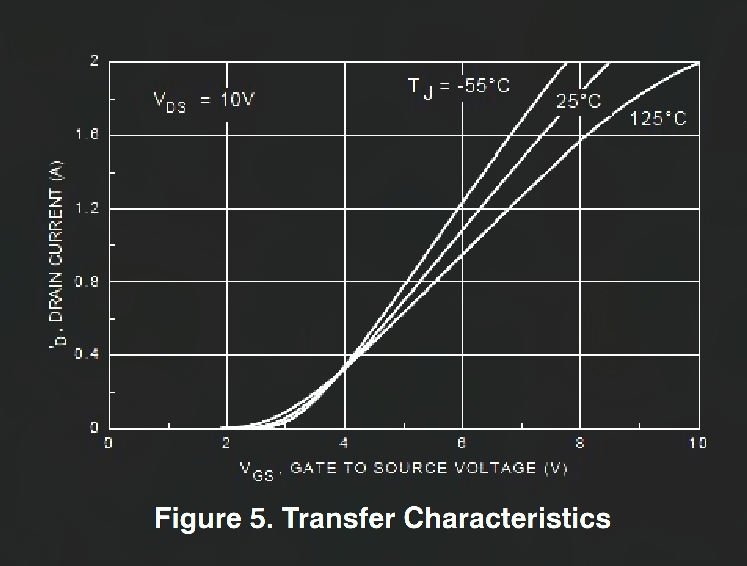
\includegraphics[width=0.5\textwidth]{Figure5.jpg} % Ajusta el tamaño con width
    \label{fig:transfer_characteristics}
\end{figure}





Para rellenar los datos \( V_T \) y \( K \) en el ejercicio, necesitamos obtener algunos valores aproximados de la gráfica para la temperatura de \( 25^\circ C \):

1. Voltaje de Umbral (\( V_T \)):
   En la gráfica, para \( T_J = 25^\circ C \), el valor de \( V_{GS} \) donde comienza a aumentar la corriente de drenaje (\( I_D \)) se encuentra aproximadamente en \( V_{GS} \approx 2.1 \, \text{V} \). Así que podemos tomar \( V_T \approx 2.1 \, \text{V} \).

2. Constante \( K \):
   Para hallar \( K \), elegimos un punto en la curva a \( 25^\circ C \). Por ejemplo, en el punto \( V_{GS} = 4 \, \text{V} \) y \( I_D = 1.2 \, \text{A} \). Sustituyendo en la ecuación \( I_D = K \cdot (V_{GS} - V_T)^2 \):

   \[
   1.2 = K \cdot (4 - 2.1)^2
   \]

   Resolviendo para \( K \):

   \[
   K = \frac{1.2}{(4 - 2.1)^2} = \frac{1.2}{3.61} \approx 0.332 \, \text{A/V}^2
   \]

Por lo tanto, los valores serían:

- \( V_T \approx 2.1 \, \text{V} \)
- \( K \approx 0.332 \, \text{A/V}^2 \)







\[
	V_T \approx 2.1 \ V \quad K \approx 0.332 \ \text{A/V}^2
\]

1) Dado el circuito de la figura 4.12, calcular el valor de \( R_D \) y \( R_S \) para cumplir las condiciones 
de polarización

Datos: \( V_D = 9\text{ V} \) e \( I_D = 6\text{ mA} \)

DATOS: \( V_{DD} = 15\text{ V} \), \( V_{SS} = -5\text{ V} \)

2) Elegir los valores de la serie normalizada E12 más próximos a los obtenidos para \( R_D \) y \( R_S \)

3) A partir de los valores nominales recalcula el punto \( Q \) y la \( g_m \)

\[
\begin{array}{|c|c|c|c|c|c|c|}
\hline
V_T & K & R_D & R_S & V_{DSQ} & I_{DQ} & g_m \\
\hline
   0 & 0 & 0 & 0 & 0 & 0 & 0 \\
\hline
\end{array}
\]





\end{document}
